\subsection{Resource Modeling}\label{subsec:resources}
\textit{(Aldo Patrone)}\quad
At every activity start the simulation must decide \emph{which} resources may
execute the activity (permissions), \emph{when} they are available
(availabilities) and \emph{which} free resource is chosen (allocation). These
three concerns are encapsulated behind a single \emph{ResourceEngine} facade:
it assigns a resource that is permitted, available and free, records it
on the event and releases it on activity completion. The selection step is a
swappable \emph{AllocationStrategy}, which is the integration point for the
optimized policies in Part~II.

\subsubsection{Resource Availabilities}
The basic model applies a fixed working interval (Mon--Fri, 08:00--18:00) to
every resource. The advanced model instead learns a \emph{per-resource calendar}:
for each resource it keeps the (weekday, hour) buckets in which that resource is
actually observed working, using a relative frequency threshold to suppress
off-hours noise. The design decision here is data-driven: BPIC-17 carries no
system-vs-human attribute and most resources act across several lanes, so a
fixed ``system always available'' rule is not supported by the data, whereas a
learned calendar per resource is. The learned calendars (Fig.~\ref{fig:availability})
cover $96.4\%$ of the real events, against $72.0\%$ for the fixed interval
(Table~\ref{tab:resource_eval}), i.e.\ they reflect real availability far more
faithfully while still constraining each resource to its own pattern. The
per-resource calendar breadth is shown in the Appendix (Fig.~\ref{fig:cal_sizes}).

\begin{figure}[!h]
    \centering
    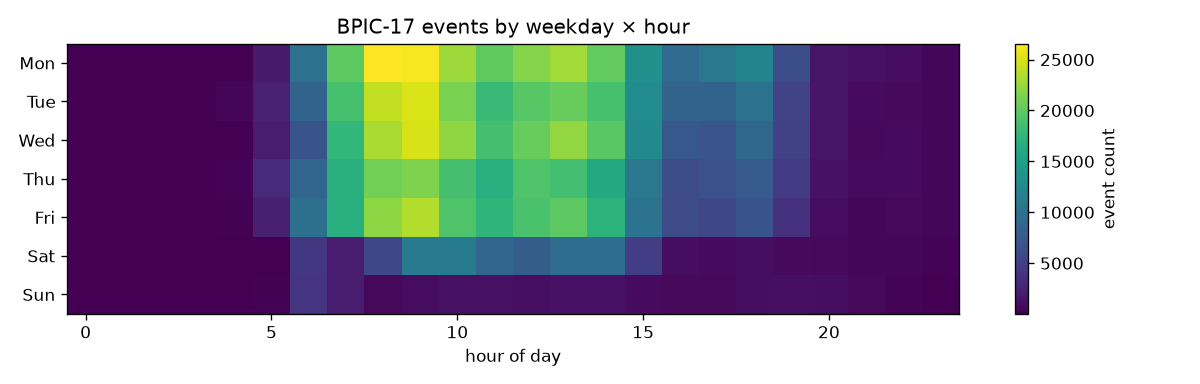
\includegraphics[width=\columnwidth]{figures/availability_heatmap.png}
    \caption{Observed BPIC-17 activity by weekday and hour. Activity concentrates
    on weekday daytime, but the fixed Mon--Fri 08--18 window only approximates the
    real pattern, motivating the learned per-resource calendars.}
    \label{fig:availability}
\end{figure}

\subsubsection{Resource Permissions}
The basic model is a resource-activity matrix: a resource may perform an
activity iff it has performed it before. The advanced model uses role
discovery with OrdinoR~\cite{yang2022ordinor}: resources are grouped into roles
and a resource may perform an activity iff its role's execution context covers
it. An observed-performer \emph{floor} is added so that every activity keeps at
least its historical executors, which guarantees that no activity becomes
unexecutable (avoiding resource deadlocks during simulation). On BPIC-17, $14$
discovered roles cover all $26$ activities and the role generalization adds
$872$ \mbox{(activity, resource)} permissions over the plain matrix, modeling
that resources within a role are interchangeable. The per-activity permission
breadth is shown in the Appendix (Fig.~\ref{fig:perm_breadth}).

\subsubsection{Resource Allocation}
Allocation selects uniformly at random among the permitted, available and free
resources. It is the deliberately unbiased Part~I baseline: it lets the other
simulation components be evaluated without an allocation policy as a confounder.
Replacing this strategy with an optimized policy is the subject of Part~II and
requires no change to the availability, permission, or core components. Its
uniformity over the candidate set is verified in the Appendix (Fig.~\ref{fig:alloc_unif}).

\begin{table}[!h]
    \caption{Resource models: basic vs.\ advanced on the real BPIC-17 log.}
    \centering
    \renewcommand{\arraystretch}{1.2}
    \footnotesize
    \begin{tabular}{lrr}
        \toprule
        \textbf{Metric} & \textbf{Basic} & \textbf{Advanced} \\
        \midrule
        Availability: event coverage      & $72.0\%$ & $96.4\%$ \\
        Permissions: activities covered    & $26/26$  & $26/26$ \\
        Permissions: role-based additions  & $0$      & $+872$ \\
        \bottomrule
    \end{tabular}
    \label{tab:resource_eval}
\end{table}
